% Created by tikzDevice version 0.10.1 on 2016-08-26 12:06:09
% !TEX encoding = UTF-8 Unicode
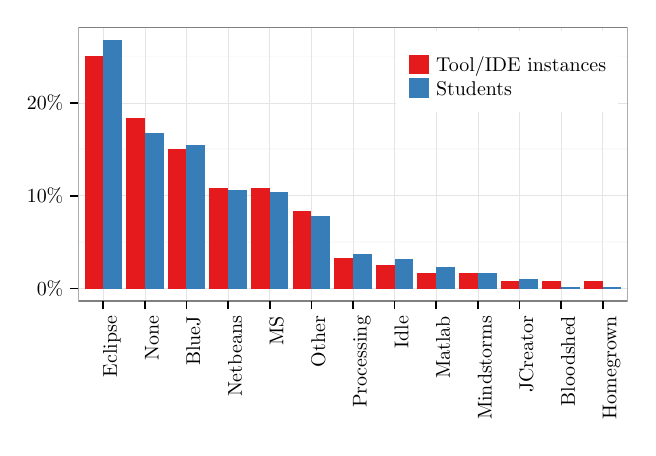
\begin{tikzpicture}[x=1pt,y=1pt]
\definecolor{fillColor}{RGB}{255,255,255}
\path[use as bounding box,fill=fillColor,fill opacity=0.00] (0,0) rectangle (216.81,144.54);
\begin{scope}
\path[clip] (  0.00,  0.00) rectangle (216.81,144.54);
\definecolor{drawColor}{RGB}{255,255,255}
\definecolor{fillColor}{RGB}{255,255,255}

\path[draw=drawColor,line width= 0.6pt,line join=round,line cap=round,fill=fillColor] (  0.00,  0.00) rectangle (216.81,144.54);
\end{scope}
\begin{scope}
\path[clip] ( 18.29, 45.74) rectangle (216.81,144.54);
\definecolor{fillColor}{RGB}{255,255,255}

\path[fill=fillColor] ( 18.29, 45.74) rectangle (216.81,144.54);
\definecolor{drawColor}{gray}{0.98}

\path[draw=drawColor,line width= 0.6pt,line join=round] ( 18.29, 67.01) --
	(216.81, 67.01);

\path[draw=drawColor,line width= 0.6pt,line join=round] ( 18.29,100.58) --
	(216.81,100.58);

\path[draw=drawColor,line width= 0.6pt,line join=round] ( 18.29,134.16) --
	(216.81,134.16);
\definecolor{drawColor}{gray}{0.90}

\path[draw=drawColor,line width= 0.2pt,line join=round] ( 18.29, 50.23) --
	(216.81, 50.23);

\path[draw=drawColor,line width= 0.2pt,line join=round] ( 18.29, 83.80) --
	(216.81, 83.80);

\path[draw=drawColor,line width= 0.2pt,line join=round] ( 18.29,117.37) --
	(216.81,117.37);

\path[draw=drawColor,line width= 0.2pt,line join=round] ( 27.31, 45.74) --
	( 27.31,144.54);

\path[draw=drawColor,line width= 0.2pt,line join=round] ( 42.35, 45.74) --
	( 42.35,144.54);

\path[draw=drawColor,line width= 0.2pt,line join=round] ( 57.39, 45.74) --
	( 57.39,144.54);

\path[draw=drawColor,line width= 0.2pt,line join=round] ( 72.43, 45.74) --
	( 72.43,144.54);

\path[draw=drawColor,line width= 0.2pt,line join=round] ( 87.47, 45.74) --
	( 87.47,144.54);

\path[draw=drawColor,line width= 0.2pt,line join=round] (102.51, 45.74) --
	(102.51,144.54);

\path[draw=drawColor,line width= 0.2pt,line join=round] (117.55, 45.74) --
	(117.55,144.54);

\path[draw=drawColor,line width= 0.2pt,line join=round] (132.59, 45.74) --
	(132.59,144.54);

\path[draw=drawColor,line width= 0.2pt,line join=round] (147.63, 45.74) --
	(147.63,144.54);

\path[draw=drawColor,line width= 0.2pt,line join=round] (162.67, 45.74) --
	(162.67,144.54);

\path[draw=drawColor,line width= 0.2pt,line join=round] (177.71, 45.74) --
	(177.71,144.54);

\path[draw=drawColor,line width= 0.2pt,line join=round] (192.75, 45.74) --
	(192.75,144.54);

\path[draw=drawColor,line width= 0.2pt,line join=round] (207.79, 45.74) --
	(207.79,144.54);
\definecolor{fillColor}{RGB}{228,26,28}

\path[fill=fillColor] ( 20.54, 50.23) rectangle ( 27.31,134.16);
\definecolor{fillColor}{RGB}{55,126,184}

\path[fill=fillColor] ( 27.31, 50.23) rectangle ( 34.08,140.05);
\definecolor{fillColor}{RGB}{228,26,28}

\path[fill=fillColor] ( 35.58, 50.23) rectangle ( 42.35,111.78);
\definecolor{fillColor}{RGB}{55,126,184}

\path[fill=fillColor] ( 42.35, 50.23) rectangle ( 49.12,106.37);
\definecolor{fillColor}{RGB}{228,26,28}

\path[fill=fillColor] ( 50.62, 50.23) rectangle ( 57.39,100.58);
\definecolor{fillColor}{RGB}{55,126,184}

\path[fill=fillColor] ( 57.39, 50.23) rectangle ( 64.16,102.25);
\definecolor{fillColor}{RGB}{228,26,28}

\path[fill=fillColor] ( 65.66, 50.23) rectangle ( 72.43, 86.60);
\definecolor{fillColor}{RGB}{55,126,184}

\path[fill=fillColor] ( 72.43, 50.23) rectangle ( 79.20, 86.04);
\definecolor{fillColor}{RGB}{228,26,28}

\path[fill=fillColor] ( 80.70, 50.23) rectangle ( 87.47, 86.60);
\definecolor{fillColor}{RGB}{55,126,184}

\path[fill=fillColor] ( 87.47, 50.23) rectangle ( 94.24, 85.00);
\definecolor{fillColor}{RGB}{228,26,28}

\path[fill=fillColor] ( 95.74, 50.23) rectangle (102.51, 78.20);
\definecolor{fillColor}{RGB}{55,126,184}

\path[fill=fillColor] (102.51, 50.23) rectangle (109.28, 76.40);
\definecolor{fillColor}{RGB}{228,26,28}

\path[fill=fillColor] (110.78, 50.23) rectangle (117.55, 61.42);
\definecolor{fillColor}{RGB}{55,126,184}

\path[fill=fillColor] (117.55, 50.23) rectangle (124.32, 62.66);
\definecolor{fillColor}{RGB}{228,26,28}

\path[fill=fillColor] (125.82, 50.23) rectangle (132.59, 58.62);
\definecolor{fillColor}{RGB}{55,126,184}

\path[fill=fillColor] (132.59, 50.23) rectangle (139.36, 61.01);
\definecolor{fillColor}{RGB}{228,26,28}

\path[fill=fillColor] (140.86, 50.23) rectangle (147.63, 55.82);
\definecolor{fillColor}{RGB}{55,126,184}

\path[fill=fillColor] (147.63, 50.23) rectangle (154.40, 58.05);
\definecolor{fillColor}{RGB}{228,26,28}

\path[fill=fillColor] (155.90, 50.23) rectangle (162.67, 55.82);
\definecolor{fillColor}{RGB}{55,126,184}

\path[fill=fillColor] (162.67, 50.23) rectangle (169.44, 55.79);
\definecolor{fillColor}{RGB}{228,26,28}

\path[fill=fillColor] (170.94, 50.23) rectangle (177.71, 53.02);
\definecolor{fillColor}{RGB}{55,126,184}

\path[fill=fillColor] (177.71, 50.23) rectangle (184.48, 53.71);
\definecolor{fillColor}{RGB}{228,26,28}

\path[fill=fillColor] (185.98, 50.23) rectangle (192.75, 53.02);
\definecolor{fillColor}{RGB}{55,126,184}

\path[fill=fillColor] (192.75, 50.23) rectangle (199.51, 50.66);
\definecolor{fillColor}{RGB}{228,26,28}

\path[fill=fillColor] (201.02, 50.23) rectangle (207.79, 53.02);
\definecolor{fillColor}{RGB}{55,126,184}

\path[fill=fillColor] (207.79, 50.23) rectangle (214.55, 50.66);
\definecolor{drawColor}{gray}{0.50}

\path[draw=drawColor,line width= 0.6pt,line join=round,line cap=round] ( 18.29, 45.74) rectangle (216.81,144.54);
\end{scope}
\begin{scope}
\path[clip] (  0.00,  0.00) rectangle (216.81,144.54);
\definecolor{drawColor}{RGB}{0,0,0}

\node[text=drawColor,anchor=base east,inner sep=0pt, outer sep=0pt, scale=  0.72] at ( 12.89, 47.75) {0\%};

\node[text=drawColor,anchor=base east,inner sep=0pt, outer sep=0pt, scale=  0.72] at ( 12.89, 81.32) {10\%};

\node[text=drawColor,anchor=base east,inner sep=0pt, outer sep=0pt, scale=  0.72] at ( 12.89,114.89) {20\%};
\end{scope}
\begin{scope}
\path[clip] (  0.00,  0.00) rectangle (216.81,144.54);
\definecolor{drawColor}{RGB}{0,0,0}

\path[draw=drawColor,line width= 0.6pt,line join=round] ( 15.29, 50.23) --
	( 18.29, 50.23);

\path[draw=drawColor,line width= 0.6pt,line join=round] ( 15.29, 83.80) --
	( 18.29, 83.80);

\path[draw=drawColor,line width= 0.6pt,line join=round] ( 15.29,117.37) --
	( 18.29,117.37);
\end{scope}
\begin{scope}
\path[clip] (  0.00,  0.00) rectangle (216.81,144.54);
\definecolor{drawColor}{RGB}{0,0,0}

\path[draw=drawColor,line width= 0.6pt,line join=round] ( 27.31, 42.74) --
	( 27.31, 45.74);

\path[draw=drawColor,line width= 0.6pt,line join=round] ( 42.35, 42.74) --
	( 42.35, 45.74);

\path[draw=drawColor,line width= 0.6pt,line join=round] ( 57.39, 42.74) --
	( 57.39, 45.74);

\path[draw=drawColor,line width= 0.6pt,line join=round] ( 72.43, 42.74) --
	( 72.43, 45.74);

\path[draw=drawColor,line width= 0.6pt,line join=round] ( 87.47, 42.74) --
	( 87.47, 45.74);

\path[draw=drawColor,line width= 0.6pt,line join=round] (102.51, 42.74) --
	(102.51, 45.74);

\path[draw=drawColor,line width= 0.6pt,line join=round] (117.55, 42.74) --
	(117.55, 45.74);

\path[draw=drawColor,line width= 0.6pt,line join=round] (132.59, 42.74) --
	(132.59, 45.74);

\path[draw=drawColor,line width= 0.6pt,line join=round] (147.63, 42.74) --
	(147.63, 45.74);

\path[draw=drawColor,line width= 0.6pt,line join=round] (162.67, 42.74) --
	(162.67, 45.74);

\path[draw=drawColor,line width= 0.6pt,line join=round] (177.71, 42.74) --
	(177.71, 45.74);

\path[draw=drawColor,line width= 0.6pt,line join=round] (192.75, 42.74) --
	(192.75, 45.74);

\path[draw=drawColor,line width= 0.6pt,line join=round] (207.79, 42.74) --
	(207.79, 45.74);
\end{scope}
\begin{scope}
\path[clip] (  0.00,  0.00) rectangle (216.81,144.54);
\definecolor{drawColor}{RGB}{0,0,0}

\node[text=drawColor,rotate= 90.00,anchor=base east,inner sep=0pt, outer sep=0pt, scale=  0.72] at ( 32.27, 40.34) {Eclipse};

\node[text=drawColor,rotate= 90.00,anchor=base east,inner sep=0pt, outer sep=0pt, scale=  0.72] at ( 47.31, 40.34) {None};

\node[text=drawColor,rotate= 90.00,anchor=base east,inner sep=0pt, outer sep=0pt, scale=  0.72] at ( 62.35, 40.34) {BlueJ};

\node[text=drawColor,rotate= 90.00,anchor=base east,inner sep=0pt, outer sep=0pt, scale=  0.72] at ( 77.39, 40.34) {Netbeans};

\node[text=drawColor,rotate= 90.00,anchor=base east,inner sep=0pt, outer sep=0pt, scale=  0.72] at ( 92.43, 40.34) {MS};

\node[text=drawColor,rotate= 90.00,anchor=base east,inner sep=0pt, outer sep=0pt, scale=  0.72] at (107.47, 40.34) {Other};

\node[text=drawColor,rotate= 90.00,anchor=base east,inner sep=0pt, outer sep=0pt, scale=  0.72] at (122.51, 40.34) {Processing};

\node[text=drawColor,rotate= 90.00,anchor=base east,inner sep=0pt, outer sep=0pt, scale=  0.72] at (137.55, 40.34) {Idle};

\node[text=drawColor,rotate= 90.00,anchor=base east,inner sep=0pt, outer sep=0pt, scale=  0.72] at (152.59, 40.34) {Matlab};

\node[text=drawColor,rotate= 90.00,anchor=base east,inner sep=0pt, outer sep=0pt, scale=  0.72] at (167.63, 40.34) {Mindstorms};

\node[text=drawColor,rotate= 90.00,anchor=base east,inner sep=0pt, outer sep=0pt, scale=  0.72] at (182.67, 40.34) {JCreator};

\node[text=drawColor,rotate= 90.00,anchor=base east,inner sep=0pt, outer sep=0pt, scale=  0.72] at (197.71, 40.34) {Bloodshed};

\node[text=drawColor,rotate= 90.00,anchor=base east,inner sep=0pt, outer sep=0pt, scale=  0.72] at (212.75, 40.34) {Homegrown};
\end{scope}
\begin{scope}
\path[clip] (  0.00,  0.00) rectangle (216.81,144.54);
\definecolor{fillColor}{RGB}{255,255,255}

\path[fill=fillColor] (132.96,114.12) rectangle (213.31,143.34);
\end{scope}
\begin{scope}
\path[clip] (  0.00,  0.00) rectangle (216.81,144.54);
\definecolor{fillColor}{RGB}{228,26,28}

\path[fill=fillColor] (137.94,127.64) rectangle (145.06,134.75);
\end{scope}
\begin{scope}
\path[clip] (  0.00,  0.00) rectangle (216.81,144.54);
\definecolor{fillColor}{RGB}{55,126,184}

\path[fill=fillColor] (137.94,119.10) rectangle (145.06,126.21);
\end{scope}
\begin{scope}
\path[clip] (  0.00,  0.00) rectangle (216.81,144.54);
\definecolor{drawColor}{RGB}{0,0,0}

\node[text=drawColor,anchor=base west,inner sep=0pt, outer sep=0pt, scale=  0.72] at (147.57,128.71) {Tool/IDE instances};
\end{scope}
\begin{scope}
\path[clip] (  0.00,  0.00) rectangle (216.81,144.54);
\definecolor{drawColor}{RGB}{0,0,0}

\node[text=drawColor,anchor=base west,inner sep=0pt, outer sep=0pt, scale=  0.72] at (147.57,120.18) {Students};
\end{scope}
\end{tikzpicture}
